\chapter{Estudo de Caso}
\label{estudo de caso}


\citeonline{wohlin2012experimentation} enuncia que é necessário que uma metodologia de estudo de caso, definida formalmente em engenharia de software, deve conter os passos da Figura \ref{fig:metodologia-estudo}.

\begin{figure}[ht!]
\centering
\includegraphics[keepaspectratio=true,scale=0.16]{figuras/metodologia-estudo-caso.eps}
\caption{Metodologia de Estudo de Caso proposta por \citeonline{wohlin2012experimentation}}
\label{fig:metodologia-estudo}
\end{figure}
\FloatBarrier

\section{Planejamento do Estudo de Caso}

Para o planejamento do estudo de caso em engenharia de software é essencial, segundo \citeonline{brereton2008using},descrever o protocolo do estudo de caso. Este consiste em um relatório simplificado das principais variáveis, dados e passos, tais como o meio e modo de coleta de dados, indetificação das fontes de dados e formas de análise de dados \cite{wohlin2012experimentation}. 


O protocolo de estudo de caso deste trabalho, que foi baseado em \citeonline{brereton2008using} e \citeonline{wohlin2012experimentation} foi dividido em seções, conforme se vê a seguir.


\subsection{Trabalhos Relacionados ao Estudo de Caso}

Assim como os trabalhos de \citeonline{Palza2003}, \citeonline{Ruiz2005}, \citeonline{Castellanos2005}, \citeonline{Becker2006}, \citeonline{Folleco2007}, \citeonline{Silveira2010}, buscou-se alcançar uma validação empírica da utilização ambiente de \textit{Data Warehousing} proposto no Capítulo \ref{chap:arquitetura}.


\subsection{Objetivos do Estudo de Caso}

O objetivo geral do estudo de caso foi avaliar um software durante o seu desenvolvimento no ambiente de \textit{Data Warehousing}. Em consonância ao objetivo geral do estudo de caso e aos objetivos específicos deste trabalho, foram definidos objetivos específicos do estudo de caso, tal como se mostra na Tabela \ref{tab:objetivos-estudo-de-caso}.

\begin{table}[H]
\begin{center}
\input{tabelas/objetivos-estudo.ltx}
\caption{Objetivos Específicos de Estudo de Caso}
\label{tab:objetivos-estudo-de-caso}
\end{center}
\end{table}
\FloatBarrier

\subsection{Seleção de Objeto do Estudo de Caso} 

Para selecionar o software que seria parte do objeto do estudo de caso considerou-se os 
critérios estábelecidos na Tabela \ref{tab:critérios-estudo-de-caso}. 


\begin{table}[H]
\begin{center}
\input{tabelas/criterios-estudo.ltx}
\caption{Critérios de Seleção de Objeto do Estudo de Caso}
\label{tab:critérios-estudo-de-caso}
\end{center}
\end{table}
\FloatBarrier

\subsection{Objeto de Estudo}

\subsubsection{Visão Geral}

O IPHAN é responsável pela gestão de diversos processos de preservação do patrimônio cultural, como por exemplo,ações para sua identificação, proteção, gestão e fomento. Decorrente
de suas atribuições, o órgão produz uma grande quantidade de informações fragmentadas em termos territoriais e temáticos. Nos últimos quatro anos, o IPHAN elaborou uma metodologia
para definir os processos de cadastro, inventário e gestão do patrimônio cultural material. Essa metodologia tem por objetivo geral abordar o Patrimônio Cultural de forma integrada, sistêmica
e estratégica, conforme detalhado a seguir:

\begin{itemize}
\item Integrada: cobrindo todas as categoriais do patrimônio material;
\item Sistêmica: estabelecendo moldes a serem utlizados nas diversas etapas de ações de preservação, possibilitando o "diálogo" e troca de informações entre áreas e etapas de trabalho;
\item Estratégica: considerando o mapeamento, a organização e a disponibilização de informações sobre o patrimônio como base para a construção de políticas públicas integradas - com outros parceiros - e de planos de preservação e desenvolvimento das regiões onde se inserem os bens.
\end{itemize}

Em termos específicos, a metodologia buscou, em primeiro lugar, mapear os procedimentos necessários para a execução das ações de cadastramento, proteção, normatização e fiscalização de bens culturais de natureza material, indicando adicionalmente os dados a serem coletados. Este mapeamento contou com a participação de representantes das Superintendências e Escritórios Técnicos, que, por meio de Grupos de Trabalho, analisaram, de forma crítica, as metodologias até então existentes.

A revisão dos processos levou à formulação da nova metodologia que, por sua vez, permitiu a otimização das atividades de cadastramento de sítios históricos e de bens tombados isoladamente e gerou a normalização das ações de fiscalização. O resultado desse trabalho produziu um conjunto de fichas e procedimentos específicos com demandas para cadastramento de dados textuais, geográficos e imagens.

Há um entendimento no IPHAN de que é necessária a formação de uma rede de proteção fomentada pelo SNPC que consolide o grande volume de informações atualmente produzido por suas unidades administrativas, composto de 27 Superintendências, 30 escritórios técnicos, 4 Unidades Especiais e 2 Parques Históricos Nacionais. Entretanto, na conjuntura atual, a natureza das informações, em grande maioria armazenadas em planilhas e em banco de dados isolados, difculta o processo de consolidação das informações, fato que frusta os esforços para a construção da rede de proteção baseada nos recursos e tecnologias atualmente adotados, pois demandaria o aporte considerável de recursos financeiros e humanos sem ganhos no processo. O órgão se manteria refém da demora na produção de informações decorrentedo intervalo entre ação e recepção das respostas, ou seja, entre a percepção do problema e sua solução.

Apesar do fato de os processos de cadastramento, normatização de sítios urbanos tombados e fiscalização de bens imóveis de metodologia já fazerem parte da realidade das Superintendências e Escritórios Técnicos, o processo manual de suporte e gestão dos dados torna a execução precária e morosa.



\subsubsection{O Software Analisado}
Tendo em vista a dificuldade que o processo manual acarreta, o IPHAN decidiu contratar uma empresa de software para desenvolver uma solução que pudesse automatizar o processo de trabalho decorrente da metodologia de inventário, cadastramento, normatização, fiscalização, planejamento e análise e gestão do patrimônio material. Esta solução de software foi concebida sobre a denominação de Sistema Integrado de Conhecimento e Gestão (SICG) que foi constuído em Java (atende-se ao critério CEC1), durante 24 releases mensais (atende-se ao critério CEC2), utilizando \textit{frameworks} como VRaptor, Hibernate formado por 7 módulos:

\begin{itemize}
\item Módulo de Conhecimento;
\item Módulo de Análise e Gestão;
\item Módulo de Cadastro;
\item Módulo de Administração de Usuários;
\item Módulo de Fiscalização;
\item Módulo de Cadastro Auxiliares;
\item Módulo de Relatórios Adicionais.
\end{itemize}


\subsection{Dados, Fonte dos Dados e Forma de Análise dos Dados}

Os principais dados quantitativos e qualitativos foram identificados na Tabela \ref{tab:dados-estudos}.

\begin{table}[H]
\begin{center}
\input{tabelas/dados-estudo.ltx}
\caption{Dados do Estudo de Caso}
\label{tab:dados-estudos}
\end{center}
\end{table}
\FloatBarrier

\subsection{Validade do Estudo de Caso}

\subsection{Limitação do Estudo de Caso}

\section{Execução do Estudo de Caso e Análise dos Dados}


Para cada uma das releases do SICG, coletou-se o código-fonte, conforme a disponibidilidade, em um servidor FTP cedido pelo IPHAN. Em alguns casos, o próprio IPHAN não possuía o código-fonte de uma determinada release tal como se mostra na Figura \ref{fig:repositorio-IPHAN}.

\begin{figure}[ht!]
\centering
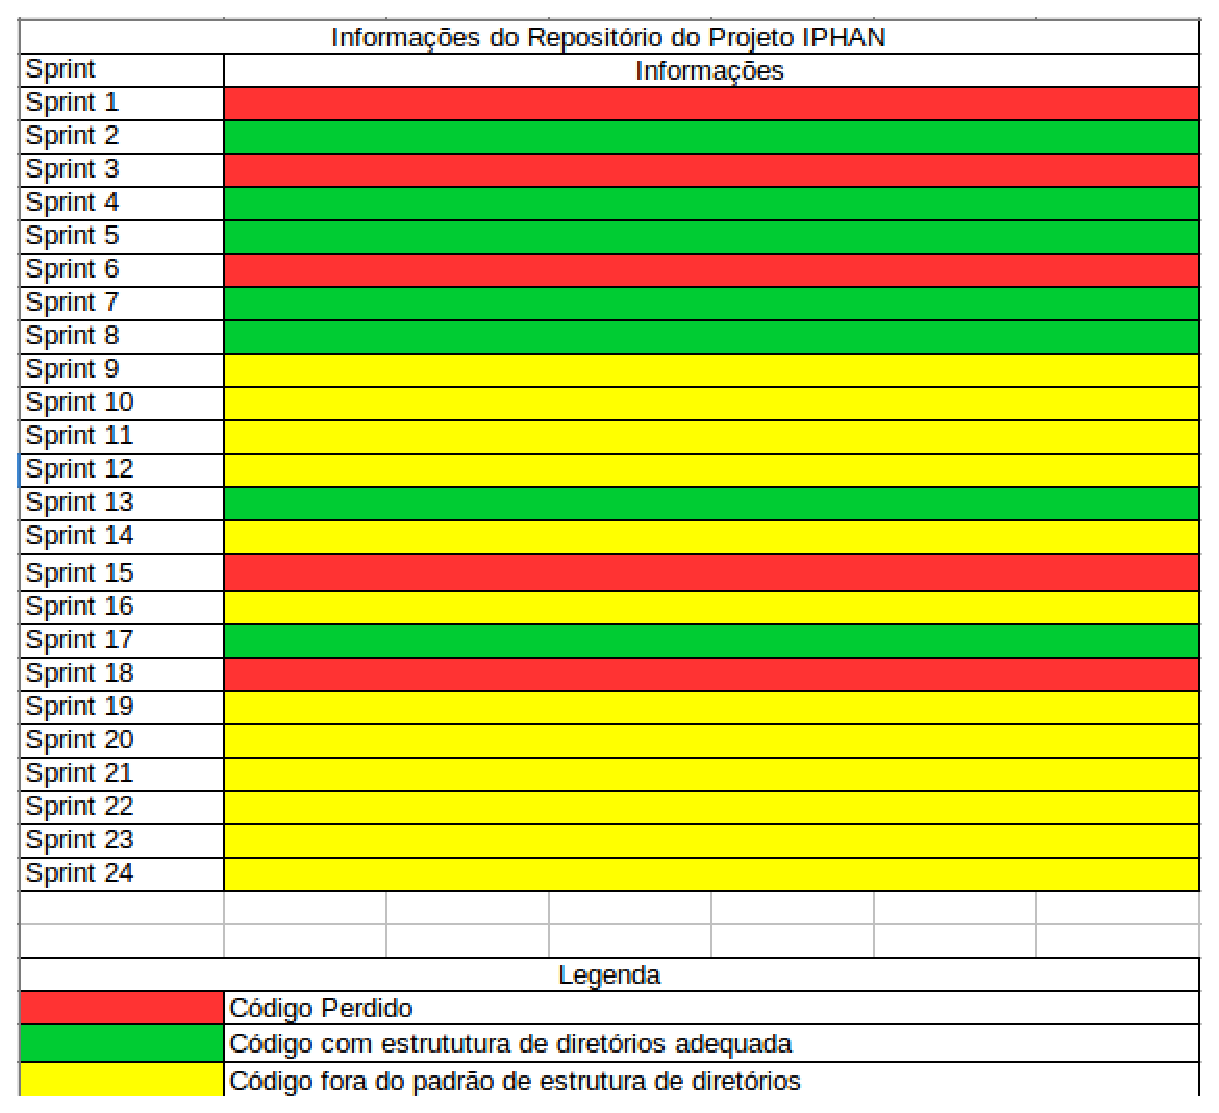
\includegraphics[keepaspectratio=true,scale=0.5]{figuras/repositorio-iphan.eps}
\caption{Informações do Repositório de Código-Fonte}
\label{fig:repositorio-IPHAN}
\end{figure}
\FloatBarrier


Após o código-fonte de cada versão ser coletado, foi feita uma análise da estrutura de diretórios, a fim de obter uma padronização na análise das métricas de código-fonte. Em casos que foram marcados com amarelos conforme a Figura \ref{fig:repositorio-IPHAN}, a estrutura de diretórios não estava condizente com a adotada, sendo necessário a correção para que as ańálises de código-fonte pudessem ser executadas corretamente para que os dados das métricas de código-fonte pudessem posteriormente ser caregados no ambiente de \textit{Data Warehousing} proposto no Capítulo \ref{chap:arquitetura}. Dessa forma, foi possível obter para cada release: Valor Percentil das Métricas de Código-Fonte para cada uma das, Quantidade de Cenários de Limpeza presentes em uma determinada Classe do Projeto e o cálculo da Taxa de Aproveitamento de Oportunidade de Melhoria de Código-Fonte. 


\subsection{Análise dos Valores Percentis para Métricas de Código-Fonte do SICG}


\subsection{Análise dos Cenários de Limpeza identificados no SICG}

\subsection{Análise da Taxa de Aproveitamento de Oportunidade de Melhoria de Código-Fonte}
